% ============================================================
% Section 2: Systematic Review of Literature
% Structured according to PRISMA guidelines and NCA journal standards.
% ============================================================

\section{Systematic Review of Literature}\label{sec:literature_review}

The intersection of computational intelligence, metaheuristic optimization, and financial time-series forecasting has generated an extensive body of literature over the past decade \cite{henrique2019stock_review, rajwar2023exhaustive_review, jiang2021applications}. Comprehensive surveys have categorized machine learning applications in financial prediction \cite{henrique2019stock_review, jiang2021applications}, systematically reviewed metaheuristic search paradigms such as Particle Swarm Optimization \cite{gad2022pso_comprehensive, wang2018pso_comprehensive} and Grey Wolf Optimizer \cite{faris2018gwo_review}, and benchmarked neural forecasting architectures under computational constraints \cite{dhingra2025solar, jovanovic2024wann}. However, despite substantial published progress in premier neural computing journals \cite{billah2024nca_moving_average, bandgar2025finchronos, al_bannoud2026accelerating, bashir2026evobagnet}, existing reviews and empirical benchmarks have not systematically evaluated the interaction between equal-budget metaheuristic tuning, temporal validation integrity, and out-of-sample trading performance. This section presents a Systematic Review of Literature (SRL) guided by the Preferred Reporting Items for Systematic Reviews and Meta-Analyses (PRISMA) protocol \cite{page2021prisma}, examining prior work across feature selection, model backbones, metaheuristic search, and validation protocols, synthesizing current state-of-the-art contributions and formalizing the three critical methodological gaps that motivate our benchmark framework.

\subsection{Literature Selection Protocol and Research Questions}\label{subsec:selection_protocol}

To ensure methodological rigor and eliminate reporting bias, relevant literature was retrieved following an explicit PRISMA search protocol across major scholarly databases: IEEE Xplore, Scopus, Web of Science, and SpringerLink (specifically targeting \textit{Neural Computing and Applications}). The search was executed using the following structured Boolean query:
\begin{itemize}
    \item (\texttt{"metaheuristic"} OR \texttt{"genetic algorithm"} OR \texttt{"particle swarm"} OR \texttt{"grey wolf"})
    \item AND (\texttt{"feature selection"} OR \texttt{"technical indicators"} OR \texttt{"Information Gain"})
    \item AND (\texttt{"futures market"} OR \texttt{"intraday forecasting"} OR \texttt{"trend classification"})
\end{itemize}

The review was bounded to peer-reviewed journal articles and top-tier conference proceedings published between 2019 and 2026. Candidate studies were screened against explicit eligibility criteria:
\begin{itemize}
    \item \textbf{Inclusion Criteria}: (i) evaluation of automated feature selection or metaheuristic hyperparameter tuning on financial or complex time-series classification/forecasting; (ii) explicit disclosure of validation protocols and search space boundaries; and (iii) reporting of empirical predictive or out-of-sample financial metrics.
    \item \textbf{Exclusion Criteria}: Studies lacking reproducible experimental parameters, omitting candidate evaluation budget details, or failing to disclose optimization constraints were excluded.
\end{itemize}

Figure~\ref{fig:prisma_flowchart} depicts the complete PRISMA literature selection workflow. The systematic review is organized around three central Research Questions (RQs):
\begin{enumerate}
    \item \textbf{RQ1 (Budget Parity)}: How do stochastic metaheuristic search operators (RS, GA, PSO, DE, GWO) compare across distinct classifier backbones (RF, SVM, MLP, 1D-CNN) when restricted to a strictly equal candidate evaluation budget cap ($N_{\mathrm{eval}} = 1{,}000$)?
    \item \textbf{RQ2 (Temporal Leakage)}: What is the quantitative impact on out-of-sample generalization when comparing chronological sequential temporal splits against randomized cross-validation on high-frequency financial time series?
    \item \textbf{RQ3 (Economic Alignment)}: How effectively do the MCC/$F_1$ and weighted-accuracy validation fitness objectives align with out-of-sample intraday trading metrics (net return, Sharpe ratio, and maximum drawdown) under exchange transaction costs?
\end{enumerate}

\begin{figure}[htbp]
\centering
\resizebox{0.92\linewidth}{!}{%
\begin{tikzpicture}[
  node distance=0.8cm and 1.0cm,
  every node/.style={
    draw=black!80,
    rounded corners=2.5pt,
    align=center,
    font=\footnotesize,
    inner sep=6pt
  },
  stage/.style={fill=black!6, text width=4.0cm, minimum height=1.1cm},
  criteria/.style={fill=black!2, text width=5.6cm, align=left},
  arrow/.style={-{Stealth[length=2.2mm]}, thick}
]

  % Nodes
  \node[stage] (db) {\textbf{Electronic Database Search}\\IEEE Xplore, Scopus,\\Web of Science, SpringerLink (NCA)};
  \node[stage, right=1.2cm of db] (retrieved) {\textbf{Identification Phase}\\$N = 1{,}248$ candidate records\\retrieved via Boolean query};
  
  \node[criteria, below=0.8cm of retrieved] (prisma) {
    \textbf{PRISMA Screening \& Eligibility Audit}\\[2pt]
    \textbf{Inclusion Criteria}:
    \begin{itemize}
      \item Peer-reviewed publications (2019--2026).
      \item Feature selection / metaheuristic tuning on financial time series.
      \item Disclosed search bounds \& validation split.
    \end{itemize}
    \textbf{Exclusion Criteria}:
    \begin{itemize}
      \item Unconstrained/undefined evaluation budget.
      \item Non-reproducible experimental parameters.
    \end{itemize}
  };
  
  \node[stage, left=1.2cm of prisma] (final) {\textbf{Included Studies}\\$N = 15$ representative studies\\+ Present Work audited in Table~\ref{tab:literature_gap}};

  % Arrows
  \draw[arrow] (db) -- (retrieved);
  \draw[arrow] (retrieved) -- (prisma);
  \draw[arrow] (prisma) -- (final);

\end{tikzpicture}%
}
\caption{PRISMA literature selection protocol flowchart mapping database retrieval, eligibility criteria filtering, and final synthesis of 15 representative studies audited in Table~\ref{tab:literature_gap}.}
\label{fig:prisma_flowchart}
\end{figure}


\FloatBarrier

\subsection{Classifier Backbones and Input Representations}\label{subsec:backbones_features}

The quality and information density of the input representation are central determinants of supervised intraday trend prediction \cite{singh2022feature}. Open, high, low, close, and volume observations encode the market state, but short-horizon bars are also affected by microstructural noise, regime shifts, and high variance. For this reason, financial machine-learning studies commonly transform raw bar data into technical descriptors representing complementary aspects of price behaviour: momentum, trend, dispersion, and volatility \cite{billah2024nca_moving_average, hunter1986exponentially, bollinger1992using}. Such representations do not create information; rather, they provide a structured hypothesis space through which a learner can test whether recent price and volume dynamics carry directional content.

The expansion of the indicator set must nevertheless be controlled. Indicators derived from common prices and overlapping lookback windows are often strongly correlated, so a large technical library can amplify redundancy, increase estimation variance, and make model ranking sensitive to incidental patterns in the development sample \cite{lei2012feature, kumar2014feature}. Feature selection is therefore a component of model design rather than a preliminary convenience: it reduces the dimensionality exposed to subsequent learning and hyperparameter search, while retaining descriptors with a demonstrable association with the target. Information Gain (IG) is a transparent filter criterion for this purpose, ranking candidate indicators by their reduction of class uncertainty \cite{lei2012feature, anonymous2025precursor}. Although a univariate ranking does not guarantee an optimal multivariate subset, its low computational cost and auditability make it appropriate for constructing a compact technical representation. The mathematical formulation and empirical application of IG in the present benchmark are detailed in Section~\ref{sec:featureselection}.

The literature spans several classifier families whose distinct inductive biases make a single preferred backbone unlikely across all market representations:
\begin{itemize}
    \item \textbf{Ensemble decision trees}, represented by Random Forest (RF), aggregate decorrelated trees built from bootstrap samples and randomly selected feature subsets. Their partition-based structure accommodates non-linear interactions and can be relatively robust to noisy descriptors \cite{nabipour2020predicting}.
    \item \textbf{Kernel margin classifiers}, represented by Support Vector Machines (SVM), seek separating hyperplanes with a maximum-margin principle. Kernel mappings, including the radial-basis-function kernel, permit non-linear decision surfaces while retaining a well-defined optimization objective \cite{naik2019optimal}.
    \item \textbf{Feedforward neural networks}, represented by Multilayer Perceptrons (MLP), learn non-linear mappings through stacked fully connected layers and backpropagation. Their expressive capacity is accompanied by sensitivity to architectural and regularization choices \cite{ecer2020mlp_ga_pso}.
    \item \textbf{One-dimensional convolutional neural networks} (1D-CNN) apply shared local filters to ordered input windows. This construction can capture short-range patterns while using parameter sharing to constrain the number of learned weights \cite{bandgar2025finchronos, dhingra2025solar}.
\end{itemize}

These families therefore represent different hypotheses about how directional information is encoded. Their comparative use is more informative than selecting a single algorithm a priori, particularly because changes in feature representation and hyperparameterization can alter the observed ranking of classifiers \cite{nabipour2020predicting, mutinda2026hybrid}. The specific representations, search domains, and fitted architectures adopted in this study are defined in Section~\ref{sec:methods}.

\subsection{Metaheuristic Optimization Paradigms}\label{subsec:metaheuristic_paradigms}

Hyperparameter selection is naturally formulated as a black-box optimization problem. Let $\boldsymbol{\theta} \in \Omega$ denote a feasible model configuration, where $\Omega$ can contain continuous, integer, categorical, and conditional variables. A validation criterion $f(\boldsymbol{\theta})$ is obtained only after fitting and evaluating the corresponding learning pipeline, and the search objective is
\begin{equation}\label{eq:metaheuristic_objective}
\boldsymbol{\theta}^{\star} = \underset{\boldsymbol{\theta} \in \Omega}{\operatorname{arg\,max}}\; f(\boldsymbol{\theta}).
\end{equation}
Unlike weight training, this objective need not be differentiable with respect to $\boldsymbol{\theta}$. Tree depth, number of hidden units, kernel choices, and regularization settings may also be discrete or conditionally active. Population-based metaheuristics are consequently attractive because they navigate such mixed spaces without gradient information and can balance broad exploration against local refinement \cite{jovanovic2024wann, faris2018gwo_review, rajwar2023exhaustive_review}.

In this context, a “candidate evaluation” should mean one complete configuration assessment under an unchanged validation protocol. This distinction is important: iterations and generations are internal counters, whereas the number of evaluated candidates is the common computational unit through which heterogeneous search procedures can be compared.

Figure~\ref{fig:backbone_optimizer_taxonomy} provides a compact taxonomy of the learning and search families considered in this literature. It distinguishes the classifier hypothesis spaces from the mechanisms used to select their configurations, while retaining the shared objective of validation-based model selection.

\begin{figure}[htbp]
\centering

\resizebox{0.96\linewidth}{!}{%
\begin{tikzpicture}[
    node distance=8mm and 10mm,
    every node/.style={
        font=\footnotesize,
        align=center
    },
    root/.style={
        draw=black!70,
        fill=black!6,
        rounded corners=2pt,
        minimum width=4.8cm,
        minimum height=0.85cm,
        font=\bfseries\footnotesize
    },
    family/.style={
        draw=black!70,
        fill=blue!18,
        rounded corners=2pt,
        minimum width=3.8cm,
        minimum height=0.78cm,
        font=\bfseries\footnotesize
    },
    classifier/.style={
        draw=black!70,
        fill=black!3,
        rounded corners=2pt,
        text width=2.05cm,
        minimum height=1.35cm,
        inner sep=4pt
    },
    search/.style={
        draw=black!70,
        fill=orange!18,
        rounded corners=2pt,
        text width=3.05cm,
        minimum height=1.25cm,
        inner sep=4pt
    },
    connector/.style={
        draw=black!65,
        line width=0.55pt
    }
]

% ============================================================
% Root
% ============================================================

\node[root] (root)
{Validation-based model selection};

% ============================================================
% Main families
% ============================================================

\node[family, below left=13mm and 15mm of root]
(backbones)
{Predictive backbones};

\node[family, below right=13mm and 15mm of root]
(searchfam)
{Search paradigms};

% Root branch
\coordinate (rootjunction) at ($(root.south)+(0,-5mm)$);

\draw[connector]
(root.south) -- (rootjunction);

\draw[connector]
(backbones.north) |- (rootjunction);

\draw[connector]
(searchfam.north) |- (rootjunction);

% ============================================================
% Predictive backbones
% ============================================================

\node[classifier, below left=12mm and 3mm of backbones]
(rf)
{\textbf{Random Forest}\\
Tree ensemble\\
and random subspaces};

\node[classifier, below right=12mm and 3mm of backbones]
(svm)
{\textbf{SVM}\\
Kernel-margin\\
classification};

\node[classifier, below=9mm of rf]
(mlp)
{\textbf{MLP}\\
Feedforward\\
neural mapping};

\node[classifier, below=9mm of svm]
(cnn)
{\textbf{1D-CNN}\\
Local filters over\\
ordered windows};

% Central backbone structure
\coordinate (backboneTop)
    at ($(backbones.south)+(0,-6mm)$);

\coordinate (backboneBottom)
    at ($(mlp.north)!0.5!(cnn.north)+(0,5mm)$);

\draw[connector]
(backbones.south) -- (backboneTop);

\draw[connector]
(backboneTop) -- (backboneBottom);

\draw[connector]
(rf.north) |- (backboneTop);

\draw[connector]
(svm.north) |- (backboneTop);

\draw[connector]
(mlp.north) |- (backboneBottom);

\draw[connector]
(cnn.north) |- (backboneBottom);

% ============================================================
% Search paradigms
% ============================================================

\node[search, below=12mm of searchfam]
(rs)
{\textbf{Random Search}\\
Uniform sampling of\\
feasible configurations};

\node[search, below=7mm of rs]
(evo)
{\textbf{Evolutionary search}\\
GA: selection, crossover, mutation\\
DE: differential variation};

\node[search, below=7mm of evo]
(swarm)
{\textbf{Swarm intelligence}\\
PSO: personal/global best\\
GWO: leader hierarchy};

% Vertical search spine
\coordinate (searchTop)
    at ($(searchfam.south)+(-2.15cm,-5mm)$);

\coordinate (searchBottom)
    at ($(swarm.west)+(-5mm,0)$);

\draw[connector]
(searchfam.south)
-- ++(0,-5mm)
-| (searchTop);

\draw[connector]
(searchTop)
-- (searchBottom |- searchTop)
-- (searchBottom);

\draw[connector]
(searchTop |- rs.west) -- (rs.west);

\draw[connector]
(searchTop |- evo.west) -- (evo.west);

\draw[connector]
(searchTop |- swarm.west) -- (swarm.west);

\end{tikzpicture}%
}

\caption{
Conceptual taxonomy linking predictive backbones with
hyperparameter-search strategies in the reviewed literature.
The left branch denotes alternative classifier hypothesis spaces,
whereas the right branch distinguishes unguided sampling,
evolutionary search, and swarm intelligence.
The precise search domains and experimental controls are
specified in Section~\ref{sec:methods}.
}
\label{fig:backbone_optimizer_taxonomy}

\end{figure}

Evolutionary algorithms maintain a population of candidate configurations and improve it through selection and variation. Genetic Algorithms (GA) emulate selection, crossover, and mutation: configurations with stronger fitness are preferentially retained or recombined, while mutation introduces new material into the population \cite{goldberg1989ga, jovanovic2024wann}. This representation-agnostic cycle is well suited to mixed hyperparameter spaces after appropriate encoding and constraint handling.

Differential Evolution (DE) is also population based, but creates candidate displacements from scaled differences between population members. A canonical donor-vector form is
\begin{equation}\label{eq:de_mutation}
\mathbf{v}_{i}^{t} = \mathbf{x}_{r_1}^{t} + F\left(\mathbf{x}_{r_2}^{t} - \mathbf{x}_{r_3}^{t}\right),
\end{equation}
where $r_1$, $r_2$, and $r_3$ index distinct population members and $F$ scales the differential displacement. Crossover then combines the donor with a target vector, and selection retains the better candidate \cite{storn1997de}. The use of population differences gives DE a self-adaptive search scale, although its practical behaviour still depends on encoding, bounds, and the chosen mutation and crossover strategy.

Swarm methods update candidates by combining individual experience with population-level information. In Particle Swarm Optimization (PSO), each particle has a position $\mathbf{x}_{i}^{t}$, a velocity $\mathbf{v}_{i}^{t}$, a personal best position $\mathbf{p}_{i}^{t}$, and an incumbent swarm-best position $\mathbf{g}^{t}$. Its standard update is
\begin{align}
\mathbf{v}_{i}^{t+1} &= \omega\mathbf{v}_{i}^{t} + c_{1}r_{1}\left(\mathbf{p}_{i}^{t}-\mathbf{x}_{i}^{t}\right) + c_{2}r_{2}\left(\mathbf{g}^{t}-\mathbf{x}_{i}^{t}\right), \label{eq:pso_velocity}\\
\mathbf{x}_{i}^{t+1} &= \mathbf{x}_{i}^{t} + \mathbf{v}_{i}^{t+1}, \label{eq:pso_position}
\end{align}
where $\omega$ controls inertia, $c_{1}$ and $c_{2}$ weight cognitive and social attraction, and $r_{1},r_{2}$ are random variates. This formulation makes the exploration--exploitation trade-off explicit and is the foundation for the broad family of PSO variants reviewed by Gad \cite{kennedy1995pso, gad2022pso_comprehensive}.

Grey Wolf Optimizer (GWO) uses a different collective metaphor. Candidate solutions are ranked into leading $\alpha$, $\beta$, and $\delta$ wolves, while the remaining wolves update their positions by encircling and approaching these leaders. Its control schedule progressively shifts the search from exploration to exploitation \cite{faris2018gwo_review, al_bannoud2026accelerating}. Despite distinct metaphors, PSO and GWO share the same benchmarking requirement: each update must be translated into feasible configurations and assessed under the same validation rule.

Random Search (RS) is an indispensable baseline because it samples feasible configurations without an adaptive search trajectory. It establishes whether the additional mechanisms of evolutionary or swarm search improve solution quality beyond unguided sampling from the same search space \cite{bergstra2012random_search}. A credible comparison must therefore control the parameter domain, candidate-evaluation count, validation data, random replication, and reporting metrics. Equalizing only the nominal number of generations or iterations is insufficient when algorithms evaluate different numbers of candidates per update.

The comparative evidence also highlights recurring weaknesses: unequal computational budgets can confound search quality with search effort; randomized validation can compromise temporal integrity; and classification-only reporting may not establish economic value after transaction costs \cite{ecer2020mlp_ga_pso, bandgar2025finchronos, billah2024nca_moving_average}. These issues are synthesized in Section~\ref{subsec:comparative_synthesis}; the concrete controls used by the present benchmark are specified only in Section~\ref{sec:methods}.


\subsection{Comparative Synthesis of Representative Studies}\label{subsec:comparative_synthesis}

To establish the state of the art and pinpoint persistent methodological gaps, Table~\ref{tab:literature_gap} synthesizes 15 representative published studies from 2019 to 2026 alongside the present benchmark work. Studies are evaluated across six technical dimensions: Study \& Year, Application Domain \& Data, Model Backbones, Optimization \& Feature Paradigms, Validation Protocol, and Identified Methodological Gap.

\begin{table}[!htbp]
\caption{Systematic Literature Review comparison matrix auditing representative studies in financial machine learning, metaheuristic hyperparameter tuning, and temporal validation protocols against identified methodological gaps.}
\label{tab:literature_gap}
\centering
\manuscripttablestyle
% Footnotesize is retained for this dense full-width synthesis matrix.
\footnotesize
\begin{tabularx}{\linewidth}{@{}>{\raggedright\arraybackslash}p{0.18\linewidth} >{\raggedright\arraybackslash}p{0.22\linewidth} >{\raggedright\arraybackslash}p{0.29\linewidth} >{\raggedright\arraybackslash}X@{}}
\toprule
Study \& Year & Domain and models & Optimization, features, and validation & Primary methodological gap \\
\midrule
Nabipour et al.\ (2020) \cite{nabipour2020predicting} & Stock-index trend; RF, SVM, ANN, XGBoost & Technical indicators; train/test split & No metaheuristic hyperparameter tuning. \\
Jovanovic et al.\ (2024) \cite{jovanovic2024wann} & Crop yield; weight-agnostic neural networks & Metaheuristic tuning; train/test & Non-financial domain; no equal-budget financial benchmark. \\
Naik \& Mohan (2019) \cite{naik2019optimal} & NSE equities; ANN classifier & Boruta feature selection; train/test & Static parameters; no metaheuristics. \\
Ecer et al.\ (2020) \cite{ecer2020mlp_ga_pso} & Financial trend; MLP & GA and PSO tuning; $K$-fold CV & Unconstrained budget; single classifier. \\
Billah et al.\ (2024) \cite{billah2024nca_moving_average} & Intraday equities; heuristic models & Moving-average rules; standard split & No neural hyperparameter tuning. \\
Bareket \& P{\^a}rv (2024) \cite{bareket2024adaptive} & Surge detection; adaptive ML & Technical indicators; medium-term split & Evaluation restricted to static features. \\
Bandgar et al.\ (2025) \cite{bandgar2025finchronos} & Financial forecasting; ensembles & Default tuning; random split & No evaluation budget cap; temporal leakage risk. \\
Rahim et al.\ (2025) \cite{rahim2025technical} & 5-min futures; single neural model & Single GA; train/test split & Single GA; no multi-optimizer benchmark. \\
Dhingra et al.\ (2025) \cite{dhingra2025solar} & Solar PV; LSTM, CNN-LSTM & RAdam, Lookahead, Adam; sequential split & Non-financial domain; stochastic optimizers omitted. \\
Mutinda \& Yong (2026) \cite{mutinda2026hybrid} & Financial market; ensembles & SEDT feature selection; $K$-fold CV & Feature selection without tuning. \\
Simatupang et al.\ (2026) \cite{simatupang2026stock} & IDX stock index; Bayesian RF & Bayesian optimization; random $K$-fold CV & Random CV risks temporal information leakage. \\
Al Bannoud et al.\ (2026) \cite{al_bannoud2026accelerating} & Kinetics series; ANN--ODE surrogate & GWO, PSO, GA, ABC; multi-partition & Non-financial; unconstrained search budget. \\
Bashir et al.\ (2026) \cite{bashir2026evobagnet} & NSE equities; bagging ensemble & (1+1) evolutionary algorithm; train/test & Single EA; no budget cap. \\
\textit{[Anonymized Precursor A]} (2025) \cite{anonymous2025precursor} & Intraday B3 futures; RF & InfoGain + default RF; sequential 60/20/20 & Untuned baseline; no metaheuristics. \\
\textit{[Anonymized Precursor B]} (2026) \cite{anonymous2026precursor} & Intraday B3 futures; MLP, SVM, RF & InfoGain + single GA; 5-fold CV & Single GA; unconstrained generation budget. \\
\textbf{Present Work} & \textbf{Intraday B3 futures; MLP, SVM, RF, 1D-CNN} & \textbf{InfoGain + RS, GA, PSO, DE, GWO; sequential 60/20/20} & \textbf{Equal $N_{\mathrm{eval}}=1{,}000$, 3 seeds, fee backtest.} \\
\botrule
\end{tabularx}
\end{table}
\FloatBarrier

As synthesized in Table~\ref{tab:literature_gap}, three primary methodological flaws permeate the existing literature on metaheuristic financial forecasting:
\begin{enumerate}
    \item \textit{The Budget Inequality Flaw}: Prior studies routinely compare metaheuristics without enforcing a strict candidate evaluation cap ($N_{\mathrm{eval}}$). Because stochastic optimization performance scales with function evaluations, superiority claims in unconstrained studies often reflect unequal computational budgets rather than algorithmic search efficiency \cite{dhingra2025solar, ecer2020mlp_ga_pso}.
    \item \textit{The Temporal Data Leakage Flaw}: Financial machine learning research frequently relies on randomized $K$-fold cross-validation or data shuffling \cite{simatupang2026stock, makridakis2018statistical}. Shuffling sequential intraday price bars allows future market information to contaminate historical training folds, yielding artificially inflated predictive accuracy scores that collapse during live execution.
    \item \textit{The Classification-Economic Disconnect Flaw}: Hyperparameter tuning is overwhelmingly conducted against raw accuracy or cross-entropy loss \cite{chicco2020mcc, anonymous2025precursor}. In high-frequency futures trading, raw accuracy ignores class imbalance and trade execution costs. A classifier achieving high nominal accuracy can incur net financial losses once exchange transaction fees and slippage are deducted.
\end{enumerate}

Figure~\ref{fig:literature_scope_by_year} shows the distribution of the 15 representative studies by publication year and optimizer-comparison scope. 

\begin{figure}[htbp]
\centering
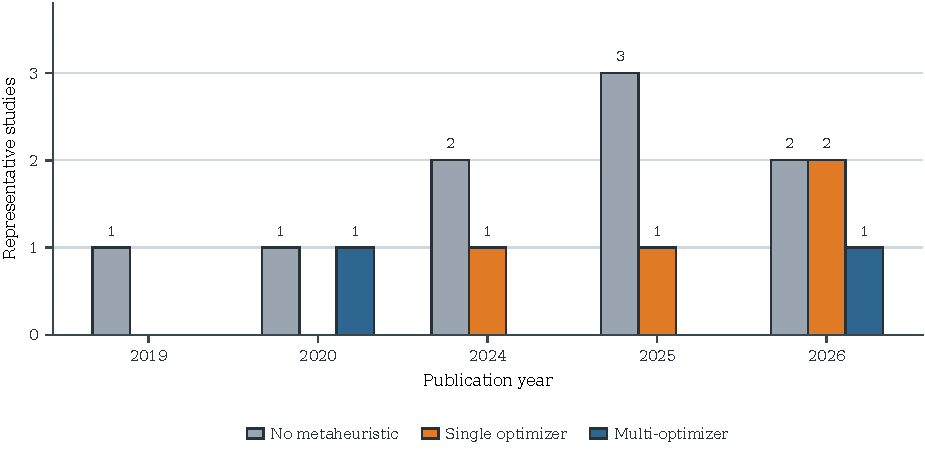
\includegraphics[width=0.90\linewidth]{figures/literature_scope_by_year.pdf}
\caption{Distribution of the 15 representative prior studies included in the literature synthesis, grouped by publication year and the scope of optimizer comparison. A study is assigned to one category according to its primary experimental design; the present work is excluded. The limited number of multi-optimizer studies motivates the controlled benchmark developed in this paper.}
\label{fig:literature_scope_by_year}
\end{figure}

\subsection{Research Positioning and Study Contribution}\label{sec:research_positioning}

The literature synthesis reveals that prior studies have typically addressed only subsets of the experimental problem considered here. Existing financial forecasting research has investigated feature selection, individual predictive models, or isolated metaheuristic tuning strategies, but these components are rarely evaluated simultaneously under common temporal and computational controls. The precursor studies in this research line first established the value of Information Gain feature selection for B3 Mini-Index futures and subsequently explored Genetic Algorithm-based hyperparameter tuning. The present work moves beyond these isolated stages by treating model selection and optimizer behaviour as components of a unified comparative benchmark.

The methodological extension is therefore not limited to increasing the number of models or optimization algorithms. The proposed framework changes the experimental control structure by combining four heterogeneous predictive backbones with five search strategies under a common feature representation, identical temporal partitions, and an equal objective-function evaluation budget. It further evaluates how optimizer behaviour changes under alternative validation objectives and complements predictive metrics with convergence analysis, matched statistical testing, and economic evaluation under transaction costs.

This design allows the study to distinguish performance differences associated with optimizer behaviour from those induced by model architecture, validation objective, or unequal search effort. Accordingly, the contribution is positioned as a controlled and reproducible model--optimizer benchmark for intraday financial classification rather than as an incremental extension of a single metaheuristic method.
